\documentclass[../../thesis]{subfiles}

\begin{document}

\section{Problem Description}
\begin{itemize}
    \item A supervised machine learning task $T$, which can be solved with a model $M$, when trained with data $D$.
    \item There are different groups of people $A$ and $B$ with different demands for the model, which they can express as set of constraints $S$ named $S_A$ in case of $A$ and $S_B$ in case of $B$. 
    \item A constraint $C \in S$ is of the form $\forall i: V(x_i) \implies y_i$, where $V(x_i)$ is an expression, which can be modelled as a SHACL Shape Network.
\end{itemize}

\section{An example for the actual state}
\begin{enumerate}
    \item Group $A$: Given $T$, $M$ is trained using the data $D_A \subseteq D$, to approximate a function $f$ by $f_A$. The constraints of $A$ are only modelled implicitly through the data $D_A$ used by group $A$. The data set $D_A \subseteq D$ may be created by manual inspection of the data, which results in a cleaning process which transforms $D$ into $D_A$.

    \item Group $B$: They receive the trained model $M$ from group $A$ and uses the model, but without knowing the constraints $S_A$ implicitly encoded through training. There is no easy way for them to validate that the model also follows their constraints $S_B$. 
\end{enumerate}

\section{Problems}
\begin{enumerate}
    \item[\textbf{Assumptions}] The cleaning / data collection process is performed by Group $A$ is made by hidden assumptions ($S_A$), which should be made explicit. Also when using such a big amount of data the cleaning process may have been performed sloppy.
    
    \item[\textbf{Validation}] Group $B$ may assume that their constraints $S_B$ are met by the model without actual performing a validation.
    
    \item[\textbf{Reasoning}] Given group $B$ finds out that there is a constraint $c \in S_B$, which is violated by the model. In the moment there will be no reasoning available, which traces back the decision of the model to the original data points $K \subseteq D_A \subseteq D$ or statistics which help to understand the situation.
\end{enumerate}

\section{Resulting possible goals}
\begin{enumerate}
    \item Building a validation process, which is able to check a model against given constraints $\rightarrow$ There is no more reason for $B$ to trust $A$ on the validity of the model. (\textbf{Validation}) \label{validation_process_goal}
    \begin{enumerate}
        \item A Validator for decision trees
        \item A Validator for random forests
    \end{enumerate}
    This also involves defining the semantics of checking a model against the constraints e.g. 
    \begin{enumerate}
        \item The semantics of validating an example from a dataset as defined below needs to be defined. 
        \item There are no explicit datapoints in a trained model. But for example in a decision tree there are nodes, which could be interpreted as an (possible endless) set of  data points associated with that node. Alternatively speaking the feature space is divided into sub spaces at each node of the decision tree.
    \end{enumerate}
    \item Collect information/statistics during training, which allows to trace back decisions made by the model to specific constraints / data points / properties of the data used for training. (\textbf{Reasoning}) \label{reasoning_goal}
    \item Some constraint might be found during training, which are actually valid for the model. This would actually be the optimal result for an ML Model: Finding hidden patterns in the training data which are true for all (the majority of) points in the training data. Check if they can be expressed as SHACL constraints). (\textbf{Assumptions}) \label{assumptions_goal}
    \item Given that the \textbf{Assumptions} problem is solved by \ref{assumptions_goal} or by explicitly modelling the assumptions made on the data as $S_A$, there might be the a chance to check whether $S_A \implies S_B$. Furthermore one could find out what is missing in $S_A$ / not implied in $S_B$ if that's not the case.
\end{enumerate}

    \begin{figure}[H]
    \centering
    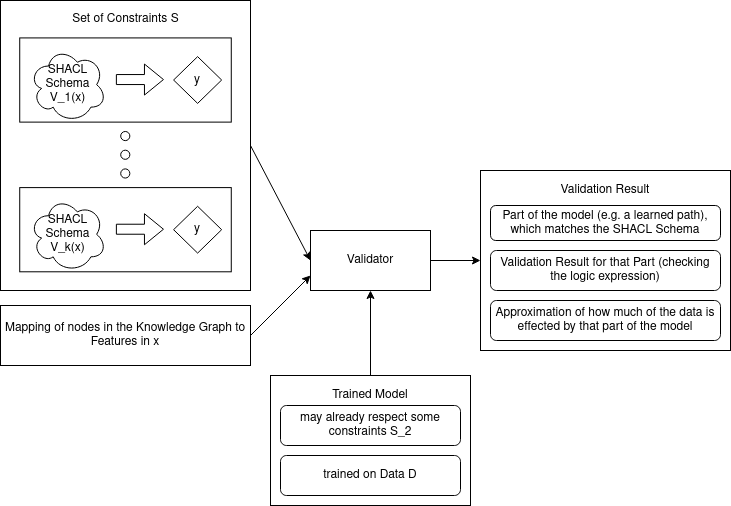
\includegraphics[width=\textwidth]{images/Validator.png}
    \caption{Sketch of a Validator}
    \end{figure}
    
\end{document}